\documentclass[en]{../../../../../../eplexam}

\usepackage{csquotes}
\usepackage[inference]{semantic}
\usepackage{placeins}
\usepackage{listings}
\usepackage{tikz}
\usetikzlibrary{automata, arrows, shapes, positioning}
\graphicspath{{img/}}


\hypertitle{Programming methods}{8}{SINF}{2224}{2016}{Juin}{All}
{Florian Thuin}
{Charles Pecheur}

\begin{abstract}
    This document is partially or totally written from sources by Gaetan Collart,
    Guillaume Kaisin and Guillaume Maudoux but in another format that didn't
    fit for git collaboration.
\end{abstract}

\section{
Describe the differences and relations between \textit{semantic proofs} and
\textit{axiomatic proofs}. Give an example of a technique belonging to each
category. Discuss their respective merits.}

\subsection{Semantic (model checking)}

In semantic, we try to prove a property based on simulation. So we need all
simulation (not always possible) to prove a validity. For example, true table
for two formula proof that they have the same semantic.

LTL properties use semantic proof, we explore every state and transitions and
then we know the property is respected or not. The main advantage: it's fully
automatic, withdraw: need to remember which state we had already visited. It
deals with loop as we remember the path.

\subsection{Axiomatic (Hoare logic)}

In axiomatic, we try to prove a property based on inference rules in order to
derive the property from the model with the assumption that the model is valid.
Example the \enquote{wp} calculus.

\subsection{Comparison}

The main advantage of the axiomatic technique is that we don't need to
simulate all the possibilities. Simulate everything is costly in time
(exponential) and in memory. \newline

A semantic proof cannot be entirely formalized in term of symbols. If every
element of the domain have a symbol and a name so the semantic proof can be
convert into an axiomatic proof.

We try to have soundness and completeness but Godel showed that it's
impossible to have both in a logic that contains arithmetic.

\clearpage
\section{
Describe the general principles of \textit{Hoare logic} (syntax and
semantics). Explain what an \textit{inference system} on this logic is, what
that is used for and how that works.}

\subsection{Definition}

Hoare logic is a formal system with a set of logic rules that allows to reason
rigorously on program correctness.

\subsection{Syntax}

The syntax is a triplet $\lbrace p\rbrace S \lbrace q\rbrace $; where $p, q$ are the pre- and
post-conditions and S is the program:

$$
\lbrace p\rbrace S \lbrace q\rbrace \iff [[S]]([[p]]) \subseteq [[q]]
$$

We have between brackets the partial correctness $\lbrace p\rbrace $ and between square
brackets the total correctness $[p]$. So we write:

\begin{eqnarray*}
  \lbrace p\rbrace S \lbrace q\rbrace & \textrm{Partial correctness} \\
  {[}p{]} S [q] & \textrm{Total correctness}
\end{eqnarray*}

\subsection{Semantics}

The intuition for semantics is that if $p$ is true, then $S$ executes, then
$q$ is true once the execution of $S$ terminates. The assertions inside $p$
or $q$ are not only simple boolean expressions, they contain first-order
assertions (predicate logic), and also equality and arithmetics.

More formally:

$$
\vDash \lbrace p\rbrace S \lbrace q\rbrace \equiv S \vDash \lbrace p\rbrace \cdot \lbrace q\rbrace
$$

$$
\vdash \lbrace p \rbrace S \lbrace q\rbrace \equiv S \vdash \lbrace p \rbrace \cdot \lbrace q\rbrace
$$

$$
\lbrace p\rbrace \cdot \lbrace q\rbrace \equiv \textrm{if p before then q after}
$$

\subsection{Logic rules (partial correctness)}

Those rules are used to reason about program correctness. They are
\enquote{complete} w.r.t an interpretation over assertions (partial
correctness). Therefore, we have a system that is coherent (an axiomatic
proof implies a semantic proof) but not complete (does not apply the other way
around).

The Hoare logic is a partial correctness logic because all true formul\ae{} are
provable from true assertion (but not necessary provable). Godel had proved that
as soon as a logic contains arithmetic it's ipossible to be sound and complete.

Inference rules of Hoare logic are used to prove validity of a program, meaning
that it respects its pre- and post-conditions. In particular, the proof can
be automated based on valid assertions (relatively complete). \newline

With these formul\ae{} we can simulate an execution and try to derive the
pre-condition from the post-condition for example (it's not whare Hoare do,
Hoare is just a logic).

To demonstrate a program, the goal is the begin with the post-conditions to
build the preconditions (left-construction proof).

\paragraph{Assignment rule}
$$
\frac{}
{ \lbrace p[E/V] \rbrace V = E; \lbrace p \rbrace }
$$

\paragraph{Consequence rule}

$$
\frac{ p \Rightarrow p' , \lbrace p' \rbrace S \lbrace q' \rbrace , q' \Rightarrow q }
{ \lbrace p \rbrace S \lbrace q \rbrace }
$$

\paragraph{Sequence rule}

$$
\frac{ \lbrace {p}_{0} \rbrace {S}_{1} \lbrace {p}_{1} \rbrace , \ldots, \lbrace {p}_{n-1} \rbrace {S}_{n} \lbrace {p}_n \rbrace }
{ \lbrace {p}_{0} \rbrace \lbrace {S}_{1} \ldots {S}_{n} \rbrace \lbrace {p}_{n} \rbrace }
$$

\paragraph{Choice rule}

We can define a \textbf{top-down} inference rule, from $p$ and $q$
(conclusion) we can build $p \land B$, $p \land \lnot B$ (premisses)

$$
\frac
{ \lbrace p \land B \rbrace S_1 \lbrace  q \rbrace , \lbrace  p \land \lnot B \rbrace  S_2 \lbrace  q \rbrace  }
{ \lbrace  p \rbrace  \textrm{ if } (B) \textrm{ then } S_1 \textrm{ else } S_2 \lbrace  q \rbrace  }
$$

There exists a \textbf{left-constructive} variant

$$
\frac
{ \lbrace  p_1 \rbrace  S_1 \lbrace  q \rbrace , \lbrace  p_2 \rbrace  S_2 \lbrace  q \rbrace  }
{ \lbrace  (B \land p_1 ) \lor (\lnot B \land p_2 ) \rbrace  \textrm{ if } (B) \textrm{ then } S_1 \textrm{ else } S_2 \lbrace  q \rbrace  \rbrace  }
$$

\paragraph{Loop rule}

$$
\frac
{ \lbrace  I \land B \rbrace  S \lbrace  I \rbrace  }
{ \lbrace  I \rbrace  \textrm{ while } (B) \textrm{ do } S \lbrace  I \land \lnot B \rbrace  }
$$

\paragraph{Reminder}

$\vdash$ is for syntaxic consequence \\
$\vDash$ is for semantic consequence \\
Soundness (all provable formul\ae{} are true): if $\vdash \lbrace p\rbrace  S\lbrace q\rbrace $ then $\vDash \lbrace p\rbrace S\lbrace q\rbrace $ \\
Completeness (all true formul\ae{} are provable): if $\vDash \lbrace p\rbrace S\lbrace q\rbrace $ then
$\vDash \lbrace p\rbrace S\lbrace q\rbrace $


\clearpage
\section{
Can one build a \textit{totally automatic} proof system for Hoare logic on a
language like Java? Discuss difficulties that occur and approaches to address
those difficulties.}

\subsection{Problem}

We can't use all rules from Hoare logic because parts of it needs elements
that can't be find easily in an automated way (e.g. variant, invariant).

\subsection{Loop}

Loop are problematic because they are based on invariant that is an assertion
to \enquote{guess}. To prove total correctness, we must also find the variant.
Without the invariant, we would have to unroll the loop infinitely, and
the resulting infinite assertion would not be well-founded. We have two rules
following the type of correctness (what follows do not work because we unroll
until the end).

\begin{description}
    \item[wlp (partial correctness):] the memory satisfies precondition $p$
    iff for any number of iterations $k$, after the execution of at least $k$
    iterations from the memory, the postcondition $q$ is satisfied.
    $$ wlp(\textrm{while }(B)\textrm{ do }S, q) \equiv \bigwedge_{k\ge 0} p_k $$
    $$ p_0 \equiv true $$
    $$ p_{k+1} \equiv (B \land wlp(S, p_k)) \lor {\lnot B \land q} $$
    \item[wp:] the set of initial states such that any execution \textbf{both}
    is non-divergent \textbf{and} terminates in a state of $Y$ (total
    correctness). The memory satisfies the precondition $p$ iff for any
    execution from the memory, there exists a number of iterations $k$, such
    that the execution terminates in less than $k$ iterations and satisfies
    the postcondition $q$
    $$ wp(\textrm{while }(B)\textrm{ do }S, q) \equiv \bigvee_{k\ge 0} p_k $$
    $$ p_0 \equiv false $$
    $$ p_{k+1} \equiv (B \land wp(S, p_k)) \lor (\lnot B \land q) $$
\end{description}

\subsection{Solution}

We can annotate the program with an invariant (invar) and a variant (bound) to
allow an automated validation.

\input{res/total_correctness_rule.tex}

\subsection{Recurrence}

Proofs can become infinite or circular. We must use a proof by total induction:

\input{res/recursive_proof_rule.tex}

\subsection{Concurrency}

Concurrency is possible with Hoare logic for disjoin parallel programs (DPP):
$$ \forall i \neq j \cdot assign(S_i) \cap var(S_j) = \emptyset $$
or if it is possible to apply proofs without interferences.

\clearpage
\section{
Make the link between resolving \textit{program proofs} and resolving
\textit{proofs in classical logic}. On that basis, explain the notion of
\textit{relative completeness} of a program proof system.}

In classical logic, we take a formula and we prove it or refutes it (or we fail
for both, then we can't conclude anything). Here, we will use an inference
system $R$ to derive theorems (proofs of programs).

Usually, in logic we have:

$$ \inference{\phi_1 \ldots \phi_n}{\phi} $$ if from all $\phi_i$, we can infer
$\phi$.

$\inference{}{\phi}$ if $\phi$ is always true (is an axiom). \newline

For program proof, we instantiate the $\phi_n$ by triplet $\lbrace p\rbrace  S \lbrace q\rbrace $. When
we derive $\phi$ in $R$, we do a proof of $\phi$. $\phi$ is a theorem of $R$
iff it exists a proof of $\phi$ in $R$.

We reduced the complex problem of program proofs to an easier problem that is
\textbf{assertions proof}.

\subsection{Relative completeness}

There exists no proof system for logic that handles arithmetics that is sound
(soundness) \textbf{and} complete (completeness) [Godel]. Here, all provable
formul\ae{} are correct (sound) but all correct formul\ae{} are not provable
(complete). However, we can have a relative completeness proving the correct
formul\ae{} from assertions that are not necessarly provable (invariant,
variant). \newline

Usually the proof that $\vDash \lbrace p\rbrace  S \lbrace q\rbrace $ is not decidable. Valid
formul\ae{} are not recursively enumerable because the existential HALT problem
can be reduce to this formula:
$$ S\textrm{ never halts iff }\vDash \lbrace true\rbrace  S \lbrace false\rbrace  $$

Invalid formul\ae{} are not decidable too because the universal HALT problem and
the first-order logic can be reduced to the formula:
$$ S\textrm{ always halts iff }\vDash [true] S [true] $$

Thus, the proof can exist but cannot be found. Approximative methods used are
decidable but are imprecise (often incomplete and sometimes incoherent).\newline

In regard of Godel theorem a logic that contains arithmetic cannot be sound
and complete. As soon as Hoare's logic allows arithmetic expression it cannot
be sound and complete. The Hoare logic is sound (hopefully) but not complete.
All true formul\ae{} can't be proved.
$$ \lbrace true\rbrace skip \lbrace P\rbrace  $$
$$ \lbrace true\rbrace  c \lbrace false\rbrace  $$

We can see that the first is valid iff the assertion $P$ is valid, the second
expression is valid iff the $c$ program don't stop so it becomes never false.
As the halt problem is not decidable, we cannot ensure that the second
expression is valid. We have a relative completeness if we have an
\enquote{oracle} (mathematical inference based on annotation) to decide
if $c$ will or not stop.

\paragraph{Reminder}

$\vdash$ is for syntaxic consequence \\
$\vDash$ is for semantic consequence \\
Soundness (all provable formul\ae{} are true): if $\vdash \lbrace p\rbrace  S\lbrace q\rbrace $ then $\vDash \lbrace p\rbrace S\lbrace q\rbrace $ \\
Completeness (all true formul\ae{} are provable): if $\vDash \lbrace p\rbrace S\lbrace q\rbrace $ then
$\vDash \lbrace p\rbrace S\lbrace q\rbrace $

\clearpage
\section{
Describe the principles of \textit{pre-condition calculus} and of generation
of \textit{verification conditions}. Explain the practical usefulness of those
computations. Make the link with Hoare logic and its inference rules.}

\subsection{Precondition calculus}

Principles of precondition calculus are WP (weakest precondition), WLP (weakest
liberal precondition) and VC (verification condition). The goal is to find the
precondition of a program based on the postcondition and on the statements
that compose the program.

\subsection{wlp calculus principle}

Technique to prove automatically a program (except while loop):

\begin{itemize}
    \item define wlp(S, q) for all kinds of statement S (program)
    \item for each case prove:
    $$ [[S]](\sigma) \subseteq [[q]] \iff \sigma \in [[wlp(S,q)]] $$
    \item we obtain a simple finite assertion in all cases (except while)
\end{itemize}

\paragraph{Explanation:} Precondition calculus is a technique that want to
derive the pre-condition based on the postcondition and the code of the program.
We can distinguish two kinds of precondition calculus. Weakest precondition
and weakest liberal precondition. The first one is the total correctness one and
the second is the partial one. \newline

We always want to find the weakest (most general) precondition to cover the
larger space. Informally, weakest, is to obtain the most generic precondition.
We can't apply it to the loop because without extra information we can't unroll
the loop without diverging because we find an infinite formula and so it's not
a well-founded assertion. Some more explanation about the loop in wp:
$$ wlp(while (B) do S, q) \equiv \bigwedge_{k \ge 0} p_k $$
$$ p_0 \equiv true $$
$$ p_{k+1} \equiv (B \land wlp(S, p_k)) \lor (\lnot B \land q) $$

But the problem is that $p_{k+1} \Rightarrow p_{k\prime} \bigwedge_{k\ge 0} p_k$
as it's an infinite formula, it's not a well-founded formula.

\subsection{Theoretical approach}

\paragraph{Weakest pre-condition} The set of initial states such that any
execution \textbf{both} is non-divergent \textbf{and} terminates in a state
of $Y$ (total correctness: non divergent and $Y$).

$$wp(S,Y) = \{\sigma \mid {[[S]]}_{\perp}(\sigma)\subseteq Y\} $$

\begin{center}
    \includegraphics[width=0.5\linewidth]{weakest_precondition.png}
\end{center}

\paragraph{Weakest liberal pre-condition} The set of initial states such
that any execution, if non-divergent, then terminates in a state of $Y$
(partial correctness: if nondivergent then $Y$):

$$ wlp(S,Y) = \{\sigma \mid [[S]](\sigma) \subseteq Y \} $$

Plus spécifiquement, le principe est de trouver les stores de la
précondition qui sera respectée par l'ensemble de stores [[p]].

$$ wlp(S, [[q]]) = \{\sigma \mid [[S]](\sigma) \subseteq [[q]] \} = [[p]] $$

\begin{minipage}{\linewidth}
    \begin{minipage}{0.45\linewidth}
        \begin{center}
            $\inference{p \Rightarrow wlp(S, q)}{\{p\} S \{q\}}$
        \end{center}
    \end{minipage}
    \begin{minipage}{0.45\linewidth}
        \includegraphics[width=0.6\linewidth]{weakest_liberal_precondition.png}
    \end{minipage}
\end{minipage}

\paragraph{Verification condition} It is what ESC/Java does. The aim is to
reduce a program to a set of assertions (=VC). To set the context, we are
here in an annotate program, it means that the author had already insert
all needed information about the loop (invariant, variant,\ldots). The syntax
of Verification Condition is:
$$ vc(p, AS, q) $$

$p$ is the precondition, AS is the annotated version of $S$, $q$ is the
postcondition. \newline

More formally, we have:
$$ \vdash [p] AS [q] \iff \vdash vc(p, AS, q) $$

and so for the relation between $AS$ and $S$
$$ \vdash vc(p, AS, q) \Rightarrow \vdash [p] S [q] $$

Warning the contrario isn't true because if we can prove a program without
annotation it doesn't imply that we can prove it with wrong annotation.\newline

We can decompose VC in two part:
$$ vc(p, AS, q) = \{p \Rightarrow vp(AS,q)\} \cup vc'(AS, q) $$

\begin{description}
    \item[vp:] that computes the precondition, approximates $wp(strip(AS), q)$.
    vp is defined exactly as wp except for loops where it's defined as:
    $$ vp(\{\textrm{invar }I\} \{\textrm{bound }E\}\textrm{ while }(B)\textrm{ do }AS, q) $$
    So it's a kind of wp which use annotated program and annotations are
    considered as valid.
    \item[vc':] it computes the internal condition, check if the annotation
    are valid.
\end{description}

VC will be used to automated to prove programs with their pre and
post-conditions, based on $wp$.

\subsection{Hoare}

We use the Hoare rules into $wp$ and so into $vc$. We use it to derive the
pre-condition from the post one with left-constructive rules and annotations
(for loop).\newline
An other link is that for a Hoare representation \{p\}S\{q\} we have that
$p = w(I)p(S,q)$

\subsection{Reminder}

Be non-divergent or terminates are two equivalent concepts but words are for
states or for traces.

\begin{description}
    \item[Termination:] last state of a non-divergent trace
    $$(S,\sigma)\textrm{ terminates in }\sigma'\textrm{ iff }(S,\sigma) \longrightarrow^{*} (\{\}, \sigma') $$
    \item[Diverges:] if the trace is infinite
    $$ (S,\sigma)\textrm{ diverges iff }(S,\sigma) \longrightarrow^{\omega} $$
\end{description}

\clearpage
\section{
Explain the notion of \textit{loop invariant} and its usefulness. Illustrate
with a proof rule. In which way does this affect automatic program proofs?
}

\subsection{Loop invariant}

It is an invariant used to prove properties on loops. Informally, an invariant
is a condition that is satisfied before and after each iteration. \newline

Without the loop invariant, we should unroll the \verb#while# loop infinitely,
resulting in an infinite precondition (thus, not well-formed). The loop
invariant is an assertion that resolves this problem: we will prove that it
is preserved by the body of the loop and we infer that the invariant is
preserved by the loop. \newline

The invariant allows to approximate the infinite assertion in a finite way
and thus by a well-formed assertion on which it is possible to reason and apply
inference rules.\newline

\subsection{Inference rule for total correctness}

The problem is that we must find $E$ and $I$.

\input{res/total_correctness_rule.tex}

\subsection{Automatic proofs}

The problem is that the loop can't be verified automatically by the $wlp$ or
$wp$ because the inference rules used is bottom up and not left-constructive.
It means that there are some elements in the premises that should be
\enquote{guessed} as for example the loop invariant and the bound (variant).
If we can't use this rule all the left-construction rules about loops lead to
an infinite derivation and so not on well-formed formula. \newline
To do so, we will use the VC calculus that uses the $wp$ and $wlp$ but also
the annotations.

For automated proofs of programs, we need to find this invariant and to prove
that it is satisfied. The problem is that an invariant cannot be found in an
automated way, so we need annotations in the programs to automate the proof.
\newline

Importance of the loop invariant is directly to apply the inference rules
(bottom-up) as a left-constructive one (yes, it's cheating). The loop invariant
represents an assertion that is true at the beginning and the end of each loop
iteration. \newline

The assertion $I \Rightarrow E \ge 0$ ensures that the variant is bounded and
as an other assertion guarantee that the bound is strictly decreasing we can derive that the loop will end. So the well-founded form of the inference rule
for the loop is:

\input{res/loop_inference_rule.tex}

We have to be careful about the trivial invariant. If the invariant is too
trivial, it will not help in the verification of the loop. Conversely, if the
invariant is too complex, the solver could not prove it (because lack of
information to prove it).\newline

The aim of the invariant as said before is to use the bottom-up rules as a
left-construction one. We have here a relative completeness as if we have
completeness with the correct annotation but we have no guarantee about the
annotation. Annotation is a kind of oracle.

\clearpage
\section{
Distinguish the notions of \textit{partial} and \textit{total correctness}.
Discuss aspects of program proofs where those notions become relevant. Explain
the notion of \textit{variant} and its usefulness, for loops and procedures.
}

\subsection{Partial correctness}

If $p$ is true before $S$ then $S$ executes and when $S$ terminates, $q$ will
be true.

$$ \vDash \{p\} S\{q\} \iff [[S]]([[p]]) \subseteq [[q]]$$

\subsection{Total correctness}

If $p$ is true, then $S$ will terminate and $q$ will be true. To have total
correctness, we must prove partial correctness \textbf{and} the termination
(variant).
$$ \vDash [p] S [q] \iff {[[S]]}_{\perp}([[p]]) \subseteq [[q]] $$

\subsection{Usefulness}

The notion of program correctness is useful to tell if an algorithm is correct
following given specifications. If the program must terminate, we use total
correctness, otherwise we use the partial correctness that ensures that the
result is correct when the program terminates.

If we have a program $S$ and a property $\phi$, we define validity of $\phi$ on
executions of $S$, they can be distinguished following partial or total
correctness.

\subsection{Variant}

The variant is an expression on enumerable set with a well-founded relation
(example: positive integers with the ascending order, string with the lexical
order,\ldots). With such relations, we can ensure that the variant decreases
at each iteration (because we can compare its new value with its old). We must
have a minimum defined by the reation to be sure that the program will
terminate. For loops, we modify the rule of Hoare logic to ensure total
correctness with a variant $E$.

\input{res/total_correctness_rule.tex}

\input{res/loop_inference_rule.tex}

For procedures, the variant is useful in case of loops or recursive procedures
(again for total correctness). We have to verify this time, that for each
recursive call, the variant decreases following the well-founded relation and
that a minimum exists. We have the following rule, $SS$ being the body of
the procedure.

\input{res/recursive_proof_rule.tex}

\clearpage
\section{
Cite and explain the proof rule for \textit{(non-recursive) procedure calls}
that corresponds to the approach used in ESC/Java. Discuss its pros and cons.
What should be modified for recursive calls?}

\subsection{Rule 1 (non-used in ESCJ)}

$$
\inference{ \{p\} \{SS\} \{q[result/V, \alpha] \} }
{ \{p[EE/VV, \alpha^{-1}]\} V=P(EE); \{q\}}
$$

\subsection{Rule 2 (used by ESCJ)}
It is used by ESCJ because the proof is done only one time (more efficient).

$$
\inference{\{p\}\{SS\}\{q\}}
{ \{p[EE/VV]\} V=P(EE); \{q[V/result, EE/VV]\} }
$$

\paragraph{Proof} We suppose a program $S$ that contains only one call to the
procedure. This procedure has a precondition and a postcondition such that
$\{p\} SS \{q\}$. To prove $S$ we use the precondition and the postcondition of
the procedure, replacing variables by the given parameters.

\paragraph{Advantages} We do the proof once for all with this rule, whereas
with rule 1 the proof has to be done at each call.

\paragraph{Drawbacks} This does not work for recursive procedures (because
it creates a circular inference, we get back to the same triplets to prove).
This rule is \textbf{not} left-constructive, it is bottom-up, so it's more
complicated (impossible without annotations) to calculate $vc$. Annotations
are mandatory, we can't guess pre- and post-condition: $p$ and $q$ must be
given as annotations.

\subsection{Recursion}

To make it work with recursive procedures, we must use complete induction,
which implies to do an hypothesis (inductive). But we also have to prove
the termination to prove total correctness. The hypothesis is that for the
recursive call, we have the pre- and post-condition satisfied. From that,
we can derive the precondition.

$$
\inference{ \{p[EE/VV]\} V=P(EE); \{q[V/result, EE/VV]\} \vdash \{p\} \{SS\}\{q\} }
{ \{p\} \{SS\} \{q\} }
$$

\input{res/recursive_proof_rule.tex}

\clearpage
\section{
Based on a simple algebraic datatype (e.g. lists), explain what is a \textit{
definition by structural induction} and discuss the advantages of such a
definition when proving programs.}

We will start with the example of the list. Here is the grammar for the list:
\begin{center}
    List = Nil $\mid$ Cons(int, List)
\end{center}

\subsection{Structural induction}

The idea is to prove proposition $P(x)$ where $x$ is an instance (of a defined
data type) defined in a recursive way with generators (see example above). A
well-founded relation is defined on the structure (as list, sub-list,
sub-sub-list, nil). A definition by structural induction is

\begin{lstlisting}[mathescape]
P(V) {
    switch(V) {
        $G_k$(V $V_k$) : $S_k$   // G(V $V_k$): S is a generator
    $\}_{k=1..n}$
}
\end{lstlisting}

The principle is that all recursive calls of $P$ in $S_k$ are of the form
$P(V_k i)$, with $V_k i \in V V_k$ ($W$ being a well-founded set, but not
$P(V))$. Thus, the property must be true for all generators to be true for
the data type of $P$. A procedure is defined by structural induction if it
respects the pattern above.

$$
\inference{
    \vdash [p \land V=Nil] \{SS\} [q], \\
    [p[V_2/V]] V' = P(V_2); [q[V'/result, V_2/V]] \vdash [p \land V = Cons(V_1,V_2)] \{SS\} [q]
} {
    [p] \{SS\} [q]
}
$$

This rule is for lists, but we have the same number of parts in the premises
than generators in the structures. \newline

Example of method that uses only generators of list and can be proved by this
technique:

\begin{lstlisting}[mathescape]
length(x) {
    switch(x) {
        case Nil: return 0;
        case Cons(n, $x_1$) : return length($x_1$) + 1;
    }
}
\end{lstlisting}

\subsection{Advantages}

Here are the different advantages given by this type of definition:

\begin{itemize}
    \item When we want to prove a procedure defined by structural induction,
    we can apply directly the inductive hypothesis. Each auxiliary proof will
    apply on a given branch of the \verb#switch#.
    \item The structure has a representation invariant (${ok}_a$). If this
    invariant is added to the precondition, then by definition of the
    structural induction, we have this invariant as postcondition. The
    invariant ${ok}_a$ defines if the structure is correct. The real advantage
    here is that there are no check to do if we know that the generator
    respects the invariant, a combination of generators will too (so it is
    structurally good).
    \item We can define the methods of production of a structure by structural
    induction by supposing that the invariant of the structure is satisfied
    for the parameters of the methods and then veryfing that the result
    of the method satisfied the invariant of the structure too.
    \item It alllows to modify a complex structure whereas variables are
    constants (e.g. delete the last element of a list).
    \item As an application, we have object-oriented programming where
    procedures are operations on the structure.
\end{itemize}

\subsection{Reminder}

$$ {\{G_k(VV_k): S_k\}}_{k=1..n} \equiv G_1(W_1): S_1 \mid \ldots \mid G_n(W_n):S_n $$

\clearpage
\section{
Based on a simple example, explain why Hoare logic proofs are \textit{not
compositional} on \textit{concurrent programs}. Succintly discuss the
particular cases of \textit{disjoint parallel programs} and \textit{
interference-free programs}.}

\subsection{Compositionalité}
Il s'agit du mécanisme selon lequel la signification d'une unité complexe est
construite à partir de la signification que ses parties ont indépendament et de
règles de combinaisons syntaxiques et sémantiques.

\subsection{Problèmes avec programmes concurrents}

Si la logique de Hoare est compositionelle avec les programmes concurrents, cela
voudrait dire qu'on peut prouver les spécifications d'un programme complexe à
partir des composantes de ce programme. Voici un exemple

\begin{lstlisting}
S_1 = {x=x+1;x=x+1;}
S_2 = {x=x+2;}
S_3 = {x=0;}
\end{lstlisting}

Si on exécute les trois S dans un système non concurrents, on n'a pas de
problèmes. Par contre, dans un système concurrents il est possible d'avoir
différents interleavings. Soit :

\begin{lstlisting}
S_A = par S_1 and S_3
S_B = par S_2 and S_3
\end{lstlisting}

On a la définition suivante (avec les modifications de mémoire)

\begin{lstlisting}
[[S_1]](n) = [[S_2]](n) = n+2
[[S_3]](n) = 0
\end{lstlisting}

Et pour les exécutions concurrentes :

\begin{lstlisting}
[[S_A]](n) = {0, 1, 2}
[[S_B]](n) = {0, 2}
\end{lstlisting}

Comme $[[S_A]](n) != [[S_B]](n)$, on dit que [[S]] est non compositionel dans le
sens où la logique de Hoare  ne nous permet pas de dériver la correction des
spécifications d'un programme concurrent en terme de spécifications locales de
ses composants sans faire référence à leur structure interne.

\begin{comment}
GM: pour être compositionnel, il faudrait pouvoir trouver f tel que [[par S1 and S2]](n) = f([[S1]](n),
[[S2]](n)) or on a [[S_B]](n) = {0,2} = f( {n+2}, {0} ) = {0, 1, 2} = [[S_A]](n), ce qui est impossible.
(f est une fonction ;­)
\end{comment}

Intuitivement, on voit qu'il n'est pas possible de réduire un programme
concurrent complexe en une suite de triplets de Hoare que l'on prouve grâce aux
règles d'inférences. En général la définition des états finaux d'un programme S
ne peut être définit en fonction de ses composantes.
Cependant, si $S_1$ et $S_2$ sont indépendants (si il ne modifient pas les mêmes
variables), on parlera de disjoint parallel programs.

Si $S_2$ n'interfere pas avec la preuve de $S_1$ (et vice versa), on parle de
interference­free proofs.

\subsection{Disjoint parallel programs}

Si on a un programme :
S = par{$S_i$}i=1..n
S est DPP si pour chaque statements parallèles $S_i$ et $S_j$s les variables utilisées par l'un ne sont
pas modifiées par l'autre. Formellement :

$$
\forall_{i\neq j} assign(S_i) \cap var(S_j) = \emptyset
$$

La règle de preuve totale est la suivante (idem pour partiel) :

$$
\inference{
    [p_1] S_1 [q_1], \ldots, [p_n] S_n [q_n]
} {
    [p_1 \land\ldots\land p_n] \mathbf{par}\{S_i\}_{i=1..n} [q_1\land\ldots\land q_n]
}
$$

Mais cela n'est pas suffisant car il est souvent impossible de trouver tous les
$p_i$ qui soient impliqués par la pré­condition p.
Il y a aussi un problème avec les variables auxiliaires. La règle des variables
auxiliaires dit que si $V$ n'est que à gauche dans les assignations et que $V$
n'apparait pas dans $q$, alors $V$ n'affecte pas le comportement de $S$. On a
donc :

$$
\inference{
    [p] S [q]
} {
    [p] S \backslash V [q]
}
$$

\begin{comment}
­­­­ seconde version ;­)
Soit in programme S tq. S = par{S_i}i=1..n
S est DPP ssi pour chaque statements parallèles S_i et S_j les variables utilisées par l'un ne
sont pas modifiées par l'autre (et vice­versa). Formellement :

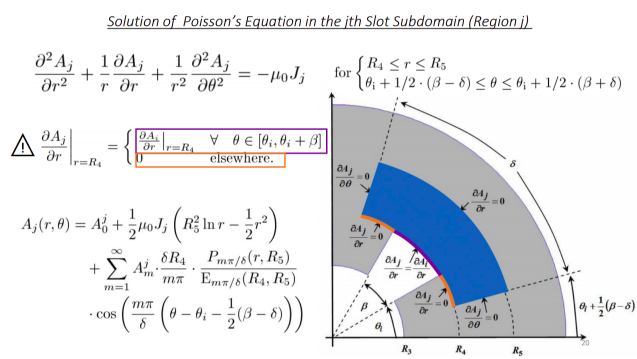
\includegraphics{4.png}

Dans ce cas, la règle d’inférence pour “par” peut se transformer de deux manières différentes
(identiques pour la partial et total correctness):
1) {p} {S_1 S_2 ... S_n} {q}
  ­­­­­­­­­­­­­­­­­­­­­­­­­­­­­­­
         {p} S {q}
Cette règle est peu intuitive, et les pré s’enchainent (la pré de S_n devient la post de S_n­1, etc).
2)

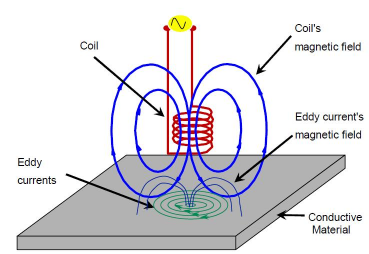
\includegraphics{5.png}

Cette règle est plus intuitive, mais pose des problèmes, car il peut être impossible de trouver
des p_i tels que p ⇒ /\ p_i.
On peut toutefois utiliser une astuce, qui consiste à introduire des variables auxiliaires.
Cette astuce résout le problème pour l’exemple donné, mais le cours ne dit pas si elle marche
toujours. Cette technique est un peu semblable aux annotation je trouve.
\end{comment}

\subsection{Interference-free proofs}

L'idée est de décomposer un programme concurrent en triplets prouvables si
chaque $S_i$ n'interfere pas avec la preuve de
$[p_j]S_j[q_j] (\forall i\neq j)$. Pour chaque triplet on doit avoir la
strong total correctness.

\paragraph{partial correctness :}
chaque statement atomique de $S_j$ préserve les assertions intermédiaires de $S_i$

\paragraph{weak total correctness :}
en plus chaque statement atomique de $S_j$ préserve le variant de la preuve de $S_i$

\paragraph{strong total correctness :}
en plus de weak, ne pas avoir de deadlocks pour les statements bloquants \enquote{choose}

\subsection{Règle}

$$
\inference{
    [p_1] S_1 [q_1 \mid \Delta], \ldots, [p_n] S_n [q_n \mid \Delta]
} {
    [p_1 \land \ldots \land p_n] \mathbf{par}\{S_i\}_{i=1..n} [q_1 \land\ldots\land q_n]
}
$$

On va donc avoir weak total correctness sur les composants et strong total
correctness sur la composition. \newline
On ne sait pas dire si c'est non­-compositionnel : cela dépend de la preuve de
chaque triplet. En complexité, les conditions sont exponentielles par rapport au
nombre de composants.


\clearpage
\section{
Describe how the notion of \textit{deadlock} occurs in program proofs. Define
\textit{strong} vs. \textit{weak} total correctness. Distinguish the case
of sequential programs (or components), then concurrent programs.}

\subsection{Deadlock}

Un deadlock est une situation où le programme $S$ est bloqué. Donc on a que,
$S'$ étant $S$ lors de son exécution, on a un $S'$ tel que $S'\neq\{\}$ et
$(S',\sigma) \nrightarrow$. La notion de blocage est différente
selon le cas d'un programme séquentiel ou concurrent.

\begin{itemize}
    \item Séquentiel : bloqué pour toujours
    \item Concurrent : bloqué mais peut être débloqué par  un autre composant concurrent.
    Bloqué pour toujours uniquement si tout les composants du programmes sont bloqués.
\end{itemize}

\begin{comment}
GM : Seuls les programmes non déterministes peuvent bloquer (instruction “choose”). Il ne faut
pas confondre les programmes séquentiels//concurrents (instruction “par”), avec les
programmes déterministes//non­déterministes (instruction “choose”).
\end{comment}

\subsection{Programmes non-déterministes (pas forcément concurrents)}
Prenons la règle du choose :

$$
\inference{
    \{p \land B_1\} S_1 \{q\}, \ldots, \{p\land B_n\} S_n \{q\}
}
{ \{p\}\mathbf{choose }\{B_i \rightarrow S_i\}_{i=1..n} \{q\} }
$$

Des deadlock peuvent se produire dans  des programmes concurrents qui
contiennent par exemple des choose dont toutes les conditions sont fausses. Il
faut donc enrichir la sémantique avec la notion de deadlock ($\Delta$). On va
définir deux nouvelles notions de correction : la correction totale forte et
faible.

\subsection{Strong total correctness}
Nouvelle sémantique :

$$
\vDash [p] S [q] \iff {[[S]]}_{\perp\Delta}([[p]]) \subseteq [[q]]
$$

On ajoute à la sémantique de S, qui est déjà étendue à la notion de divergence
($\perp$), la notion de deadlock ($\Delta$). Cette dernière peut être comprise
comme l'ensemble des assertions qui rendent le store $\sigma$ vrai et qui
permettent d'atteindre un état dans lequel il reste des statements à exécuter
et depuis lequel on ne peut plus effectuer aucune transition. Formellement :

$$
{[[S]]}_{\perp\Delta}(\sigma) = [[S]](\sigma) \cup \{\perp \mid (S,\sigma)\} \rightarrow^{\omega} \cup \{\Delta \mid (S,\sigma) \rightarrow^{*} (S',\sigma') \nrightarrow, S' \neq \{\} \}
$$

Pour la preuve, on ajoute une condition qui dit qu'il y a au moins une branche d'ouverte :

$$
\inference{
    p \Rightarrow (B_1 \lor \ldots \lor B_n) \\
    [p \land B_1] S_1 [q], \ldots, [p \land B_n] S_n [q]
} {
    [p]\mathbf{choose }{\{B_i \rightarrow S_i\}}_{i=1..n}[q]
}
$$

\subsection{Weak total correctness}
On considère les exécutions qui ne divergent pas mais qui peuvent avoir un deadlock :

$$ {[[S]]}_{\perp}(\sigma) = [[S]](\sigma) \cup \{\perp \mid (S,\sigma) \rightarrow^{\omega}\} $$

Ce qui donne :

$$ \vDash [p] S [q \mid \Delta] \iff {[[S]]}_{\perp\Delta}([[p]]) \subseteq [[q]] \cup \{\Delta \} $$

\subsection{Concurrents vs Séquentiels}

Pour un programme concurrent on pourrait avoir que le tout soit strong total et
que les composants soient weak total (deadlock débloqué par un autre sous
programme) alors qu'en programme séquentiel on ne peut avoir que l'un des deux
(strong ou weak). La décomposition restera strong ou weak en fonction de ce
qu'était le programme entier.


\clearpage
\section{
Show the principles of \textit{linear temporal logic} (LTL) and its
interpretation over Kripke structures. Describe an example of LTL property.
}

\subsection{Principes}

Les principes de LTL est de raisonner sur la succession d'états dans le temps.
On parlera d'exécutions linéaires, et donc de traces d'exécutions d'un modèle.
LTL propose les concepts suivants :

\begin{itemize}
    \item X \textcolor{green!60!black}{$p$} = \enquote{in the ne\textcolor{red!60!black}{\bf X}t state, \textcolor{green!60!black}{$p$}}

    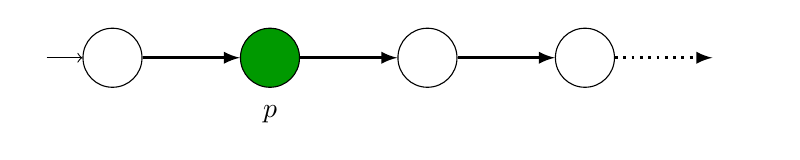
\begin{tikzpicture}[node distance=2cm]
        \node[initial, draw, circle, initial text={}, minimum width=0.75cm] (A) {};
        \node[circle,draw, right of=A, fill=green!60!black, minimum width=0.75cm] (B) {};
        \node[circle,draw, right of=B, minimum width=0.75cm] (C) {};
        \node[circle,draw, right of=C, minimum width=0.75cm] (D) {};
        \node[right of=D, minimum width=0.75cm] (E) {};
        \node[below = 0.1cm of B] {$p$};

        \path[-latex, line width=1pt] (A) edge node {} (B);
        \path[-latex, line width=1pt] (B) edge node {} (C);
        \path[-latex, line width=1pt] (C) edge node {} (D);
        \path[-latex, dotted, line width=1pt] (D) edge node {} (E);
    \end{tikzpicture}

    \item F \textcolor{green!60!black}{$p$} = \enquote{\textcolor{red!60!black}{\bf F}inally (sooner or later) \textcolor{green!60!black}{$p$}}

    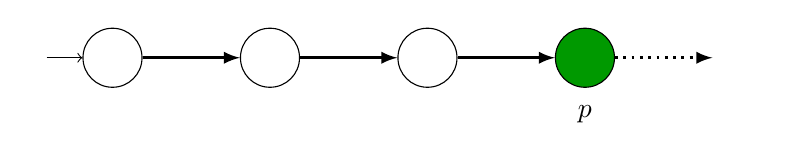
\begin{tikzpicture}[node distance=2cm]
        \node[initial, draw, circle, initial text={}, minimum width=0.75cm] (A) {};
        \node[circle,draw, right of=A, minimum width=0.75cm] (B) {};
        \node[circle,draw, right of=B, minimum width=0.75cm] (C) {};
        \node[circle,draw, right of=C, fill=green!60!black, minimum width=0.75cm] (D) {};
        \node[right of=D, minimum width=0.75cm] (E) {};
        \node[below = 0.1cm of D] {$p$};

        \path[-latex, line width=1pt] (A) edge node {} (B);
        \path[-latex, line width=1pt] (B) edge node {} (C);
        \path[-latex, line width=1pt] (C) edge node {} (D);
        \path[-latex, dotted, line width=1pt] (D) edge node {} (E);
    \end{tikzpicture}

    \item G \textcolor{green!60!black}{$p$} = \enquote{\textcolor{red!60!black}{\bf G}lobally (always) \textcolor{green!60!black}{$p$}}

    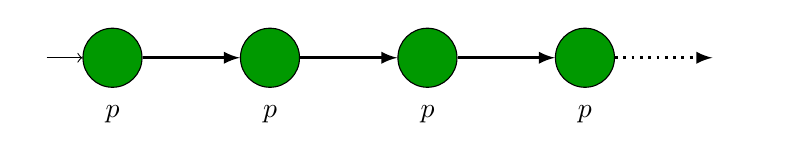
\begin{tikzpicture}[node distance=2cm]
        \node[initial, draw, circle, initial text={}, minimum width=0.75cm, fill=green!60!black] (A) {};
        \node[circle,draw, right of=A, minimum width=0.75cm, fill=green!60!black] (B) {};
        \node[circle,draw, right of=B, fill=green!60!black, minimum width=0.75cm] (C) {};
        \node[circle,draw, right of=C, minimum width=0.75cm, fill=green!60!black] (D) {};
        \node[right of=D, minimum width=0.75cm] (E) {};
        \node[below = 0.1cm of A] {$p$};
        \node[below = 0.1cm of B] {$p$};
        \node[below = 0.1cm of C] {$p$};
        \node[below = 0.1cm of D] {$p$};

        \path[-latex, line width=1pt] (A) edge node {} (B);
        \path[-latex, line width=1pt] (B) edge node {} (C);
        \path[-latex, line width=1pt] (C) edge node {} (D);
        \path[-latex, dotted, line width=1pt] (D) edge node {} (E);
    \end{tikzpicture}

    \item (\textcolor{green!60!black}{$p$} U \textcolor{red!60!black}{$q$}) = \enquote{\textcolor{green!60!black}{$p$} \textcolor{red!60!black}{\bf U}ntil \textcolor{red!60!black}{$q$} (and sooner or later \textcolor{red!60!black}{$q$})} \\
    (\textcolor{green!60!black}{$p$} W \textcolor{red!60!black}{$q$}) = \enquote{\textcolor{green!60!black}{$p$} unless \textcolor{red!60!black}{$q$} (or always \textcolor{green!60!black}{$p$})}

    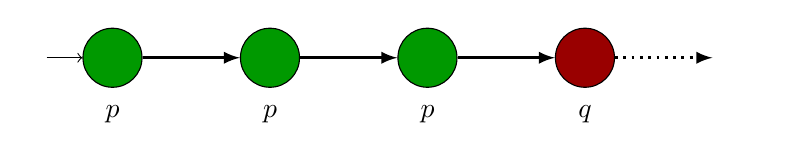
\begin{tikzpicture}[node distance=2cm]
        \node[initial, draw, circle, initial text={}, minimum width=0.75cm, fill=green!60!black] (A) {};
        \node[circle,draw, right of=A, minimum width=0.75cm,fill=green!60!black] (B) {};
        \node[circle,draw, right of=B, fill=green!60!black, minimum width=0.75cm, fill=green!60!black] (C) {};
        \node[circle,draw, right of=C, minimum width=0.75cm, fill=red!60!black] (D) {};
        \node[right of=D, minimum width=0.75cm] (E) {};
        \node[below = 0.1cm of A] (F) {$p$};
        \node[below = 0.1cm of B] (F) {$p$};
        \node[below = 0.1cm of C] (F) {$p$};
        \node[below = 0.1cm of D] (F) {$q$};

        \path[-latex, line width=1pt] (A) edge node {} (B);
        \path[-latex, line width=1pt] (B) edge node {} (C);
        \path[-latex, line width=1pt] (C) edge node {} (D);
        \path[-latex, dotted, line width=1pt] (D) edge node {} (E);
    \end{tikzpicture}
\end{itemize}

\subsection{Kripke Structures}
$$K = \langle Q, T, Q_0, P, V\rangle$$

\begin{itemize}
    \item $Q$: set of states,
    \item $T \subseteq Q \times Q$: transition relation,
    \item $Q_0 \subseteq Q$: initial states,
    \item $P$: atomic propositions,
    \item $V: Q \rightarrow 2P$: interpretation function.
\end{itemize}

Si on a une Kripke structure $K$ à laquelle appartient une trace $\pi$, pour un
état $i \ge 0$, $(K,\pi,i) \vDash \phi$ veut dire $\phi$ est vrai à l'état $i$
de l'exécution $\pi$ de $K$.\newline

On a les sémantiques suivantes :

\begin{eqnarray*}
    (K, \pi\ i) \vDash & \iff & p \in V(\pi(i)) (p \in P) \\
    (K, \pi, i) \vDash X\phi & \iff & (K, \pi, i+1) \vDash \phi \\
    (K, \pi, i) \vDash (\phi U \phi') & \iff & \exists_j i \le j \land (K,\pi,j) \vDash \phi' \land \forall_k i \le k < j \Rightarrow (K,\pi,k) \vDash \phi\\
    (K,\pi) \vDash \phi & \iff & (K,\pi,0) \vDash \phi \\
    K \vDash \phi & \iff & \forall_{\pi\in Tr(K)} (K,\pi) \vDash \phi
\end{eqnarray*}

\begin{figure}[!ht]
    \begin{center}
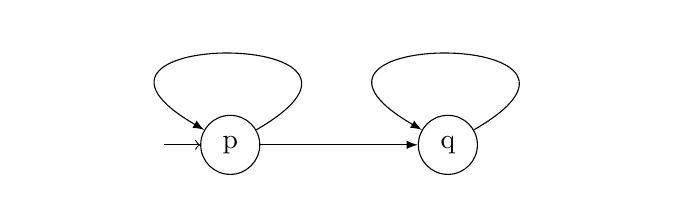
\begin{tikzpicture}
    \node[initial, circle, draw, minimum width=0.75cm, initial text={}] (p) {p};
    \node[circle, draw, right = 2cm of p, minimum width=0.75cm] (q) {q};

    \path[-latex] (p) edge node {} (q);
    \path[-latex] (p) edge [loop above, in=150, out=30, looseness=10] node {} (p);
    \path[-latex] (q) edge [loop above, in=150, out=30, looseness=10] node {} (q);
\end{tikzpicture}
    \end{center}
\caption{p U q}
\end{figure}
\FloatBarrier{}

\begin{figure}[!ht]
    \begin{center}
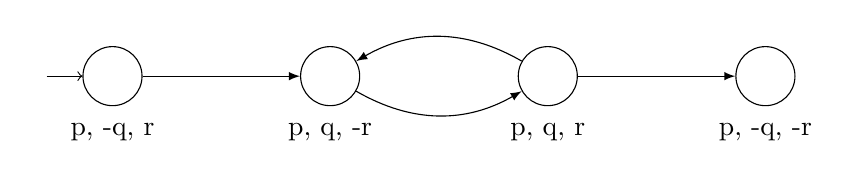
\begin{tikzpicture}
    \node[initial, circle, draw, minimum width=0.75cm, initial text={}] (A) {};
    \node[circle, draw, right = 2cm of A, minimum width=0.75cm] (B) {};
    \node[circle, draw, right = 2cm of B, minimum width=0.75cm] (C) {};
    \node[circle, draw, right = 2cm of C, minimum width=0.75cm] (D) {};
    \node[below =0.1cm of A] {p, -q, r};
    \node[below =0.1cm of B] {p, q, -r};
    \node[below =0.1cm of C] {p, q, r};
    \node[below =0.1cm of D] {p, -q, -r};

    \path[-latex] (A) edge node {} (B);
    \path[-latex] (B) edge [bend right] node {} (C);
    \path[-latex] (C) edge [bend right] node {} (B);
    \path[-latex] (C) edge node {} (D);
\end{tikzpicture}
    \end{center}
\caption{G p}
\end{figure}
\FloatBarrier{}


\clearpage
\section{
Describe the general principle of \textit{model-checking} for simple
properties (e.g. invariants). Compare with deductive proofs, in terms of
limitation, automation, kinds of properties to be checked.}

\subsection{Model checking principle}

Le principe du model checking est de vérifier qu'un modèle (e.g. une Kripke
structure) satisfait une propriété (e.g. une formule LTL) par une exploration
exaustive de tous les états du modèle. Bien que les exécutions puissent être
infinies, la vérification est finie car le modèle est fini (on ne considère que
les modèles finis, et il contient des boucles). On mémorise donc la trace
visitée afin de ne pas boucler.

\subsection{Vérification et Réfutation}
On veut vérifier que $K \vDash \phi$. Si on trouve une trace $\pi$ qui n'est pas
satisfaite, alors on a réfuté. Si on n'en a pas trouvé et que la recherche est
complète, alors $K \vDash \phi$ est vérifiée. Mais il n'est en
général pas possible d'effectuer une recherche complète.

\paragraph{Principe pour LTL}
Avec LTL le cheminement est le suivant :

\begin{enumerate}
    \item Prendre la négation de $\phi$ ($\lnot\phi$).
    \item A partir de $\lnot\phi$ on fait un automate de Buchi $B_{\lnot\phi}$
    \item On combine le model $K$ avec $B_{\lnot\phi}$
    \item On explore $K \times B_{\lnot\phi}$
\end{enumerate}

\subsection{1ere version : Reachability}

Il s'agit d'une version réduite du model­-checking. Cela renvoie un préfixe
d'exécution $\phi$ qui mène à un état $q \in A \subseteq Q$ (acceptance condition : error states). Le principe est le suivant :

\begin{enumerate}
    \item Visiter tous les états accessibles depuis $Q_0$ via une recherche DFS
    \item Mémoriser tous les états visités pour éviter de boucler
    \item Si un état $q \in A$ est trouvé alors la trace est sur la pile de la recherche DFS
\end{enumerate}

Cela permet de vérifier les propriétés safety, par exemple:

\begin{itemize}
    \item Invariants: on dit que $I$ est invariant ssi $\lnot I$ n'est pas
    atteignable
    \item Assertion: S = assert p est respectée si at $S \land\lnot p$ n'est
    pas atteignable.
    \item Exclusivité mutuelle: S et S' sont mutuellement exclusifs ssi
    at $S \land at S'$ nest pas atteignable.
\end{itemize}

\subsection{2e version : LTL}

Cette version permet de vérifier n'importe quelle propriété LTL, cela renvoie
une exécution infinie $\pi$ telle que $\pi\lnot\vDash\phi$. On va utiliser une
structure Kripke et une relation de transition $T$ totale (donc chaque état a
une transition, donc transition infinie partout). Le principe est le suivant:

\begin{enumerate}
    \item Générer $B_{\lnot\phi}$ qui accepte les exécutions qui violent $\phi$
    \item Combiner $K$ et $B_{\lnot\phi}$ dans un nouvel automate
    $K\times B_{\lnot\phi}$
    \item Rechercher une exécution acceptante dans $K \times B_{\lnot\phi}$.
    Pour cela on va utiliser le double DFS (repeated reachability). La
    complexité est de $O(\mid K \times B \mid) = O(\mid K \mid . \mid B \mid)$
\end{enumerate}

\subsection{Comparaison avec deductive proof}

\begin{tabular}{l|p{0.35\linewidth}p{0.35\linewidth}}
& \bf Model checking & \bf Deductive proof \\ \hline
\bf Space & explosion du nombre d'états & aucune \\
\bf Reactive systems & Gère les preuves & Ne gère pas les preuves \\
\bf Automation & totalement automatique & a besoin d'annotation pour les
invariants \\
\bf Properties & safety (respect d'invariant, assertion,\ldots) et LTL et liveness (buchi et double DFS) & safety mais pas LTL ni liveness \\
\end{tabular}

Si tu as par exemple \verb#while(true) x=x+1;# alors le modèle sera infini (vu
qu'on ne retombera jamais sur un état identique, la trace sera infinie). Avec
les preuves déductives il n'y a pas de cette limitation.

\clearpage
\section{
Describe the principle of \textit{model-checking for LTL} using Büchi
automata. Discuss its algorithmic complexity. Mention a method that can
improve the efficiency of model-checking.}

\subsection{Buchi automata}

Un automate de Buchi accepte des mots infinis si il existe une exécution
infinie qui visite un nombre infini de fois une condition acceptante
$F \subseteq Q$. La particularité des automates de Buchi est d'avoir des
libellés sur les transitions. On a donc $T \subseteq Q \times \sigma \times Q$
($\sigma$ étant l'alphabet). Il n'y a qu'un état initial $q_0 \in Q$.
Formellement :

$$
B = \langle \sigma, Q, T, q_0, F \rangle
$$

Il est possible de transformer n'importe quelle formule LTL $\phi$ sur $K$ en
un automate $B_{\phi}$ dont l'alphabet serait le powerset de P. La taille de
l'automate $\mid B_{\phi} \mid$ est exponentielle selon $\mid\phi\mid$ dans le
pire des cas.

\subsection{Model checking with Buchi automaton}

Le principe du model checking (LTL) est de trouver une exécution infinie $\pi$
dans $K$ telle que $\pi\lnot \vDash \phi$. Si on ne trouve pas de telle
exécution, alors échec.

\begin{enumerate}
    \item Générer un automate de Buchi $B_{\lnot\phi}$ qui accepte les
    exécutions infinies qui violent $\phi$.
    \item On combine l'automate $B_{\lnot\phi}$ avec $K$ en un nouvel automate
    $K \times B_{\lnot\phi}$
    \item Chercher une exécution infinie acceptante dans ce nouvel automate.
    Si on a une exécution finie, alors on rajoute un état $q_{\perp}$ qui a une transition vers lui-­même et on ajoute une transition vers cet état depuis tout ceux qui n'ont aucune transition sortante.
\end{enumerate}

Si on a $K = \langle Q, T, Q_0, P, V \rangle$ et
$B = \langle 2^P, Q', T', q_0', F' \rangle$ alors on peut construire
$K \times B = \langle 2^P, Q \times Q', T'', Q_0 \times \{q_0'\}, Q\times F' \rangle$
avec $(q,q') \rightarrow^{a} (q'', q''') \in T''$ ssi il y a une transition
$q \rightarrow q'' \in T$ et si $q' \rightarrow^{a} q''' \in T'$ et si $a=V(q)$.

\subsection{Repeated reachability}

\begin{enumerate}
    \item On visite tous les états atteignables depuis Q0 dans une première
    recherche (DFS1).
    \item Si DFS1 atteind un état acceptant, on visite tous les états qu'on
    peut atteindre depuis cet état (DFS2).
    \item Si DFS2 atteind une nouvelle fois l'état acceptant, alors on a une
    boucle, et une exécution acceptante est dans la stack de DFS1 (le préfixe)
    et DFS2 (la boucle).
\end{enumerate}

On peut imaginer des améliorations de cette recherche:

\begin{itemize}
    \item Stopper  le DFS2 quand on tombe sur un élément  du DFS1 (on sait que
    il existe un chemin à partir de cet élément pour revenir à l'état acceptant)
    \item Stopper le DFS2 quand on tombe sur un état visité dans un précédent
    DFS2 (vu que cet état retombe sur un état acceptant)
\end{itemize}

La recherche devient donc linéaire en fonction du nombre d'états $O(\mid Q
\mid)$

\subsection{Complexity}

Pour faire du model-­checking en utilisant les automates de Buchi, on doit
suivre ces différentes étapes:

\begin{enumerate}
    \item Création de $B_{\lnot\phi}: O(2^{\mid\phi\mid})$. \textbf{Si on a un
    nombre X de symboles} dans la formule, à chacun d'entre eux on peut avoir
    deux états (symbole=true, symbole=false), donc c'est exponentiel en
    fonction de la taille de la formule.
    \item Création de $K \times B_{\lnot\phi} : O(\mid K\mid .\mid
    B_{\lnot\phi\mid})$. On a déjà une structure de Kripke $K$ associée à la
    formule $\phi$, on doit fusionner  cette structure avec l'automate
    $B_{\lnot\phi}$ et donc vérifier chaque association d'états venant des deux
    structures. Donc la complexité est fonction de la multiplication des
    tailles des deux structures
    \item Double DFS linéaire en $O(\mid Q\mid = \mid K \times B \mid)$
    \item Donc la sortie finale du model-­checking aura la complexité $O(\mid
    K\mid . 2^{\mid\phi\mid})$
\end{enumerate}

Le plus gros problème reste l'explosion du nombre d'états de la structure de
Kripke. Si on a un programme \verb#S = par S1 and ... and Sn#. Si $\mid K(S_k)
\mid = O(m)$ alors on a que $\mid K(S) \mid = O(m^n)$ vu qu'on prend en compte
tous les entrelacements qu'il peut y avoir dans ces différentes parties de
programme. On peut imaginer plusieurs solution pour réduire cette explosion:

\begin{itemize}
    \item Partial order reduction: on considère que deux transitions
    $q_1 \rightarrow q \leftarrow q_2$ sont équivalentes si il existe $q'$ tel
    que $q_1 \rightarrow q' \leftarrow q_2$. Si deux transitions sont
    mutuellement indépendantes et qu'elles n'affectent pas la propriété
    vérifiée alors on peut considérer seulement une seule transition. Le
    problème avec cette solution est de trouver des transitions indépendantes.
    \item Symbolic model checking: on va encoder un état  comme un ensemble de
    variables binaires. On raisonne en terme de ensembles d'états (initiaux,
    d'erreurs, successeurs). De cette manière on n'énumère plus tous les états
    mais on travaille sur un ensemble d'entre eux. (cf slide 42­-43 chap 11)
    \item Bounded model-­checking: on va faire du model­checking normal sauf
    qu'on va limiter la profondeur maximale à laquelle on va explorer les
    états. On peut faire du breadth­-first pour avoir les traces les plus
    courtes, ou iterative deepening,\ldots
    \item Partial model-­checking: on va effectuer un model-­checking classique
    jusqu'a être à court de ressource.
    \item State hashing model­-checking: on définit un hash pour chaque état à
    partir des composantes de l'état. Quand on a une collision du hash les
    états sont fusionnés (de toute manière ils sont identiques). On peut
    configurer les composants sur lequel le hash se porte pour assurer que
    toutes les exécutions importantes sont vérifiées. Ce type de model­-checking
    limite le nombre d'exécution.
    \item Stateless model­-checking: on ne mémorise plus les états. Il ne nous
    reste donc plus qu'à controller les scheduling et les choix
    non-­deterministes. Le principe est qu'on mémorise les choix le long de
    l'exécution, on backtrack pour explorer les choix alternatifs (tout cela
    avec une profondeur limitée sinon on bouclerait a l'infini). On une depth
    max de D, on va mémoriser tous les choix jusqu'a la profondeur D et ensuite
    revenir a l'état D­1 et modifier le choix. On remonte donc l'arbre.
\end{itemize}

\end{document}
